
Die folgenden Regeln gelten für die zweite Edition (2nd Edition) des Spiels. Einige kleinere Abschnitte sind nicht übersetzt und mit drei Punkten … markiert. Diese Abschnitte enthalten aber keine zusätzlichen Regeln, die nicht schon anderswo erwähnt werden.

\subsection{Spielübersicht}

In dem Spiel „Betrayal at House on the Hill“ verkörpert jeder Spieler einen Charakter der ein altes, gruseliges Haus erforscht. Bei der Erforschung entdeckt man neue Räume. Immer wenn ein neuer Raum entdeckt wurde, findet man dort etwas ... oder etwas findet \emph{dich}. Die Abenteurer verbessern oder verschlechtern sich, je nachdem wie sie mit den gefundenen Überraschungen im Haus umgehen. Und in jedem Spiel ist das Haus anders aufgebaut.

Irgendwann während des Spiels löst einer der Spieler ein Ereignis aus, das HAUNT (Spuk) genannt wird. Wenn dieser Punkt eingetreten ist, wird ein Spieler allen anderen in den Rücken fallen. Dieser Charakter wird zum Verräter und wird davon besessen sein seine ehemaligen Gefährten zu bekämpfen. Die restlichen Abenteurer werden zu Helden, die versuchen das ganze Abenteuer einfach nur zu überleben. Von diesem Punkt an ist dieses Spiel ein Kampf zwischen dem Verräter und den Helden... oft auch ein Kampf um Leben und Tod.

Dieses Spiel beinhaltet 50 verschiedene Spuk-Szenarien und jedes erzählt eine andere Geschichte. Diese gilt es von Euch zu erforschen, bis zum Überleben oder Sterben, in dem \textsc{Haus auf dem Hügel}.

\subsection{Spielmaterial}

\begin{itemize}
    \item[1] Regelheft
    \item[2] Spukbücher („Buch des Verräters“ und „Geheimnisse des Überlebens“)
    \item[44] Raum-Felder
    \item[1] Eingangshallen-Feld (beinhaltet 3 Räume)
    \item[6] Charakter-Figuren aus Plastik
    \item[6] beidseitig bedruckte Charakter-Karten
    \item[30] Plastik-Clips
    \item[8] Würfel
    \item[1] Runden/Schadensanzeiger
    \item[13] Omen-Karten
    \item[22] Gegenstand-Karten
    \item[45] Ereignis-Karten
    \item[291] Papp-Marker, im Einzelnen:
    \item[12] große runde Monster-Marker (mit Gattung)
    \item[204] kleine runde Monster-Marker
    \item[14] rechteckige Ereignis- und Raum-Marker
    \item[43] fünfeckige Gegenstand-Marker
    \item[18] dreieckige Verräter-Würfel-Marker
\end{itemize}

\subsection{Ziel des Spiels}

Durchsuche das Haus und stärke Deinen Charakter bis das „Spuk-Szenario“ beginnt. Danach ist es Dein Ziel die Siegbedingung für Deine Seite als erstes zu erfüllen, entweder als Verräter oder als Held.

\subsection{Spielvorbereitung}

\begin{itemize}
    \item Lege die Bücher „Buch des Verräters“ (TRAITORS’S TOME) und „Geheimnisse des Überlebens“ (SECRETS OF SURVIVAL) zur Seite. Sie werden erst nach dem Auslösen des Spuks benötigt.
    \item Jeder Spieler sucht sich eine Charakterkarte aus. Jede Karte hat zwei Seiten. Entscheide dich für eine.
    \item Befestige 4 Plastikclips an der Karte und zwar so, das sie auf die grünen Anfangswerte der jeweiligen Eigenschaft Geschwindigkeit (\speed), Kraft (\might), Wissen (\know) und Gesundheit (\sanity) zeigen.
    \item Die Karten Omen, Item und Event werden getrennt voneinander gemischt und als verdeckte Stapel bereit gelegt.
    \item Suche die Raumkarten BASEMENT LANDING , ENTRANCE HALL / FOYER / GRAND STAIRCASE und UPPER LANDING heraus. Lege sie mit etwas Abstand zueinander auf dem Tisch aus.
    \item Mische alle restlichen Raum-Felder und lege sie als verdeckter Stapel ab. (Die Bezeichnungen auf den Rückseiten der Karten sind hier noch uninteressant.)
    \item Jeder Spieler stellt seine Figur in die ENTRANCE HALL. (Jede Figurenfarbe entspricht der Hintergrundfarbe auf der entsprechenden Charakterkarte.)
    \item Die Würfel werden griffbereit abgelegt.
    \item Ermittelt wer das Spiel beginnt. Der Charakter der als nächster Geburtstag hat beginnt (schaue auf der Charakterkarte deiner Figur nach dem Geburtstag). Danach folgen die Spieler im Uhrzeigersinn.
\end{itemize}


\subsection{Traits / Charakterwerte}

Jeder Entdecker hat vier Charaktereigenschaften (traits), die durch die vier Zahlenreihen auf der Charakterkarte dargestellt werden. Geschwindigkeit (\speed) und Stärke (\might) sind physische / körperliche Eigenschaften (physical traits). Geistige Gesundheit (\sanity) und Wissen (\know) sind mentale Eigenschaften (mental traits.)

Viele Karten beeinflussen deine Werte. Wenn ein Effekt oder Angriff deine Werte beeinflusst, verschiebe den Plastikclip um so viele Felder wie angegeben. Jede Eigenschaft hat einen Maximalwert, der nicht überschritten werden kann, auch wenn ein Effekt ihn erhöhen würde.

\begin{center}
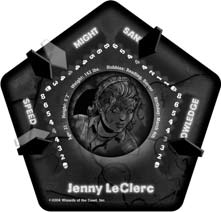
\includegraphics[width=6cm]{resources/traits}
\end{center}

Jede Eigenschaft zeigt auch ein Schädelsymbol. Sinkt eine Eigenschaft auf das Schädelsymbol nachdem der Spuk begonnen hat stirbt dein Charakter. Vor Beginn des Spuks kann niemand sterben. Jede Eigenschaft verbleibt dann immer mindestens auf der Stufe über dem Schädel, auch wenn die Eigenschaft reduziert werden müsste.

Physischer Schaden wird nach belieben zwischen \might\ und \speed\ aufgeteilt. Du bewegst die Clips so viele Stufen nach unten, wie du Schaden erlitten hast.

Mentaler Schaden wird zwischen \sanity\ und \know\ aufgeteilt.

Im Beispielbild hat Jenny 3 physischen Schaden erlitten.

\subsection{Spielablauf}

Angefangen beim Startspieler führt jeder Spieler im Uhrzeigersinn einen Entdeckungszug im Haus durch.

\subsection{Wenn du am Zug bist …}
… kannst du beliebig viele der folgenden Aktionen durchführen, egal in welcher Reihenfolge:

\begin{itemize}
    \item Du kannst dich bewegen.
    \item Du kannst einen neuen Raum entdecken.
    \item Du kannst Item- oder Omenkarten einsetzen.
    \item Du kannst würfeln.
    \item Du kannst angreifen (einmal pro Zug nachdem der Spuk begonnen hat).
\end{itemize}

Solange der Spuk noch nicht begonnen hat, musst du am Ende deines Zuges einen Spuk-Wurf machen (siehe Spuk-Wurf durchführen auf Seite \pageref{kap:rule:makehauntroll}), wenn du zuvor in dieser Runde eine Omenkarte gezogen hast. Das Spiel bekommt einige neue Wendungen sobald der Spuk beginnt (siehe in
„Der Spuk“ auf Seite \pageref{kap:rule:haunt}).


\subsubsection{Bewegen}

Wenn du am Zug bist kannst du so viele Felder weit laufen, wie es deine SPEED-Anzeige auf deiner Charakterkarte anzeigt. Du kannst Aktionen wie Angriffe oder das Benutzen eines Gegenstandes unterwegs ausführen. Wenn es sich im Spiel ergibt, dass du eine Karte ziehen musst, ist deine Bewegung für diese Runde beendet. Anderfalls darfst du weitere Räume entdecken.

\paragraph{Beispiel für eine Bewegung:} … (Stimmt nicht ganz im englischen Orginal :)

\subsubsection{Entdecken eines neuen Raumes}
\label{kap:rule:discoverroom}

Wenn deine Figur eine Tür betritt und sich auf der anderen Seite kein Raum befindet, nimm dir das oberste Feld vom Raum-Stapel. Wenn es die gleiche Etage anzeigt wie die auf der du dich gerade befindest, legst du das Feld einfach an dieser Tür an und betrittst das Feld mit deiner Figur. Lege jedes neue Raumfeld so logisch wie möglich an, so dass immer angrenzende Räume entstehen die durch die Türen verbunden werden. (Verbinde Türöffnungen immer wenn es möglich ist. Türen, die auf Wände zeigen werden zu Scheintüren.)

Falls das gezogene Raum-Feld nicht zu deiner momentanen Etage passt, lege es verdeckt auf einen Ablagestapel. Ziehe auf diese Weise so lange neue Felder nach bis ein passendes gefunden ist. (Einige Felder können auf mehreren Etagen eingesetzt werden.)

Abenteurer können nicht durch Scheintüren gehen. Scheinfenster (falsche Fenster, also Fenster mit dahinterliegender fester Wand) zählen nicht als Fenster im Sinne von offenen Fenstern bei Events oder in einer Spukbeschreibung, es sei denn es steht explizit das Gegenteil geschrieben.

Ein Abenteurer kann jederzeit durch eine Tür gehen wenn sie mit einem angrenzenden Raum verbunden ist. Türen sind immer offen. Die einzige Ausnahme bildet die Eingangstür in der ENTRANCE HALL. Sie ist immer verschlossen. Du kannst das Haus nicht verlassen es sei denn ein Spuk-Szenario erlaubt es dir. (Freiluft-Räume gehören ebenfalls zum Haus.)

Treppen verbinden Etagen miteinander. Die große Treppe im Eingangsbereich führt immer zum Obergeschoß. Die Treppen im Keller führen immer zum und vom Foyer durch eine geheime Tür. (Du kannst die Kellertreppen erst benutzen wenn du sie im Keller entdeckt
hast.)

Einige Räume haben bestimmte Auswirkungen auf deinen Charakter, wenn er diesen Raum betritt. Auf manche Raumkarten sind spezielle Regeln aufgedruckt, die beim Eintreten oder Verlassen aktiviert werden. Gehören zu einem Raum sowohl ein Regeltext als auch ein Symbol, wird die entsprechende Karte zuerst gezogen und ausgeführt.

Manche Räume beeinflussen auch die Bewegung. Einige besondere Räume sind auch noch mal in dem Abschnitt „Spezielle Räume“ auf Seite \pageref{kap:rules:specialrooms} erklärt.


\subsubsection{Kann ich ein Stockwerk durch das Legen eines neuen Raumes abschließen?}

Nein, du darfst Räume nicht so anlegen, dass alle Türen in dem Stockwerk miteinander verbunden sind. Wenn es keine bessere Anlegestelle für einen Raum gibt, ziehe eine andere Raumkarte, solange, bis du eine findest, die eine Tür frei lässt. Gibt es keine Raumkarte mehr, mit der dies möglich ist, ordne die bestehenden Räume so um, dass es wieder offene Türen gibt.

\subsubsection{Was passiert, wenn der Raumstapel leer ist?}

Mische die Karten, die du beim Benutzen des Raumstapels beiseitegelegt hast und fange erneut mit diesen an.

Gibt es überhaupt keine Räume für ein Stockwerk mehr, hast du das Stockwerk / Haus vollständig entdeckt.

\subsubsection{Ziehen von Omen-, Gegenstand- oder Ereigniskarten}

Ein gezogenes Raum-Feld kann ein Kartensymbol enthalten. Wenn du das erste Mal einen Raum mit einem Kartensymbol ziehst, endet dein Zug in diesem Raum und du ziehst die entsprechende Karte. Nur der erste Spieler, der einen Raum betritt, zieht eine Karte.

Wenn der Raum ein Spiral-Symbol hat, ziehst du eine EVENT-Karte. Lese sie laut vor und folge den Anweisungen die auch beinhalten können, dass du würfeln musst. Danach wird die Karte abgelegt falls dort nichts Gegensätzliches angegeben ist oder die Karte noch weiterführende Auswirkungen hat.

Wenn der Raum ein Stierkopf-Symbol hat, ziehst Du eine ITEM-Karte. Sie wird laut vorgelesen und offen vor dir abgelegt; somit hast du diesen Gegenstand in deinem Besitz. Du kannst ihn sofort und pro Zug einmal benutzen wenn nichts anderes auf der Karte
angegeben ist.

Wenn der Raum ein Raben-Symbol hat, ziehst du eine OMEN-Karte. Lies sie laut vor und lege sie dann offen vor dir ab. Es kann sein das du nun sofort etwas tun musst. Am Ende deines Zuges musst Du auf jeden Fall einen „Spuk-Wurf“ durchführen, wenn der Spuk noch nicht begonnen hat (Seite \pageref{kap:rule:makehauntroll}).

Wenn du aufgrund eines Effektes einen neuen Raum ziehen musst, und dieser neue Raum ein Symbol hat, ziehst du die entsprechende Karte. Wird ein Raum aus anderen Gründen angefügt, z.B. wegen Anweisungen im Spukbuch, zieht der erste Spieler, der diesen Raum betritt, keine Karte.

Auch wenn deine Bewegung mit dem Ziehen einer Karte endet, kannst du immer noch Gegenstände benutzen, angreifen, …

\subsubsection{Spezielle Räume}
\label{kap:rules:specialrooms}

Viele Räume haben Besonderheiten die auf dem Feld angegeben sind. Einige von ihnen haben aber auch noch spezielle Eigenschaften die hier aufgelistet werden:

\paragraph{CHASM, CATACOMBS, THE VAULT und TOWER}

Dies sind alles Sperr-Räume. Eine Sperre kann verhindern, dass du den dahinter liegenden Raum betrittst. Um ihn zu durchqueren muss man einen auf dem Feld angegebenen Wurf durchführen. Diesen Wurf kannst du einmal pro Runde versuchen. Das Durchqueren der Sperre kostet keinen Bewegungspunkt. Wenn der Wurf misslingt, musst du stehen bleiben. In deinem nächsten Zug kannst du es erneut versuchen oder du gehst den Weg zurück auf dem du gekommen bist.

Abenteurer können nicht mit anderen Abenteurern, die sich auf der anderen Seite einer Sperre aufhalten, interagieren oder sie angreifen. Monster ignorieren Sperren, aber wenn ein Monster seine Bewegung in einem Sperr-Raum beendet muss der Verräter entscheiden, auf welcher Seite der Sperre das Monster anhält.

Wenn ein Effekt dich in einem Sperr-Raum absetzt, kannst du entscheiden, auf welcher Seite du landest. Wenn ein Marker in dem Raum abgelegt werden muss (z.B. Geheimgang), bleibt dieser Marker dauerhaft auf der gewählten Seite.

\paragraph{ENTRANCE HALL (Die Eingangshalle) \& Co.}

Die Eingangshalle, das Foyer und die große Treppe befinden sich alle auf einem Feld gelten aber trotzdem als drei verschiedene Räume. THE GRAND STAIRCASE und UPPER LANDING gelten als zwei verschiedene Räume.


\paragraph{THE COAL CHUTE (Der Kohlenschacht)}

Betrete den Kohlenschacht, um mit einem Schritt zum BASEMENT LANDING zu kommen. Ein Zug eines Entdeckers oder Monsters kann nicht auf dem Kohlenschacht enden. (Die Figur landet automatisch im BASEMENT LANDING .)

\paragraph{THE COLLAPSED ROOM (Der zusammengefallene Raum)}

Nur der Spieler der als erstes diesen Raum entdeckt muss den dort angegebenen „Geschwindigkeits-Wurf“ ausführen. Danach können alle Spieler die diesen Raum betreten dies ignorieren, allerdings können sie es auch ausführen. In diesem Fall muss der Spieler aber auch den evtl. Schaden in Kauf nehmen. Das Herunterfallen in den Keller zählt nicht als Schritt für die Bewegung, der Spieler nimmt trotzdem Schaden.

Nur der erste Spieler, der in das Loch fällt, wählt ein Keller-Feld und legt es an. Auf dieses Feld wir dann der Marker BELOW COLLAPSED ROOM abgelegt und jeder weitere Spieler der herunterfällt landet in diesem Raum. Lege das neue Keller-Feld an die bestehenden Kellerräume an. Gibt es keine Kellerräume mehr, wähle einen bestehenden Raum als Zielraum aus.

Ist der erste Charakter, der den eingestürzten Raum betritt, ein Monster, setze das Monster in einen beliebigen Kellerraum und ziehe keinen neuen Raum.

\paragraph{JUNK ROOM (Rumpelkammer)}

Bremst dich dieser Raum beim Verlassen und deine verbleibende Bewegung würde dich am Verlassen hindern, kommst du dennoch heraus. Du bleibst im Nachbarraum stehen.

\paragraph{THE MYSTIC ELEVATOR (Der mysteriöse Fahrstuhl)}

Dieses Feld bewegt sich, sobald es betreten wird. Würfel mit zwei Würfeln und lege dieses Feld an eine Tür der erwürfelten Etage an. (Wenn sich dort keine befindet bleibt der Fahrstuhl dort wo er ist.) Wenn du die Etage erwürfelst, auf der du dich gerade befindest, kannst du ihn an eine andere Tür dieser Etage legen. Der Fahrstuhl kann nur einmal pro Zug benutzt werden.

Monster und der Verräter können das Fahrstuhlziel ohne zu würfeln beliebig wählen. Der Fahrstuhl kann sich jedoch nur einmal pro Verräterzug inklusive aller Monsterzüge bewegen. In anderen Worten: Verwendet der Verräter den Fahrstuhl für seine Figur, funktioniert er nicht mehr, wenn Monster im folgenden Monsterzug den Fahrstuhl benutzen wollen.

Ein Held muss den Fahrstuhlwurf ausführen, sobald er den Fahrstuhl betritt oder wenn er seinen Zug ohne Bewegung im Fahrstuhl verharrt hat.

Wenn sich mehrere Spieler im Fahrstuhl aufhalten, und ein anderer Spieler tritt ein und würfelt eine 0, nehmen alle Spieler im Fahrstuhl schaden.

Wenn ein Effekt in den Fahrstuhl führt (z.B. der eingestürzte Raum oder der Geheimgang), verbleibt der entsprechende Marker im Fahrstuhl, auch wenn sich dieser bewegt.

\paragraph{THE VAULT (Der Tresorraum)}

Landet ein Spieler durch einen Effekt in diesem Raum, befindet er sich außerhalb der verschlossenen Tür. Sobald das Gewölbe einmal geöffnet wurde, wird der Marker EMPTY VAULT dort abgelegt. Der Verräter öffnet den Tresor nicht automatisch, er muss zum Öffnen auch den Wurf bestehen.

%\paragraph{THE CRYPT (Die Gruft)}
%
%Monster ignorieren die Auswirkungen dieses Raumes.
%
%\paragraph{THE FURNACE ROOM (Der Heizraum)}
%
%Monster ignorieren die Auswirkungen dieses Raumes.

\subsubsection{Benutzen von Gegenstand- und Omenkarten}
\label{kap:rule:useitemomen}

Alle Abenteurer können ihre Gegenstände einmal pro Zug benutzen. Manche Monster können das ebenfalls, wenn die Spukregeln es erlauben. Die meisten Omen-Karten (ausgenommen der Karte BITE) sind ebenfalls Gegenstände, die man nehmen und benutzen kann wie ITEM-Gegenstände. Es gibt keine maximale Anzahl an gleichzeitig tragbaren Gegenständen.

Einmal während deines Zuges kannst du (oder ein Monster) folgendes tun:
  \begin{itemize}
    \item Einen Gegenstand einem anderen Mitspieler geben, der sich im selben Raum wie du befindet (wenn beide einverstanden sind).
    \item Gegenstände fallen lassen. (Wenn du das tust, musst du einen fünfeckigen ITEM-Marker im Raum ablegen.) Ein anderer Spieler oder auch du selbst, kann diesen Gegenstand (oder auch mehrere gleichzeitig) später aufheben.
    \item Hebe einen oder mehrere Gegenstände aus dem Raum auf. Entferne die Marker entsprechend.
\end{itemize}

Einige Gegenstände können nicht getauscht werden. Sie können jedoch abgelegt und aufgehoben werden. Der Text auf der Karte gibt an, ob eine solche Aktion verboten ist.

Der Hund, der Biss, das Mädchen und der Verrückte sind keine richtigen Gegenstände und können daher nicht getauscht, gestohlen oder abgelegt werden.

Mit jedem Gegenstand kann ein Spieler \emph{eine} der folgenden Aktionen pro Runde durchgeführen:

  \begin{itemize}
        \bitem Den Gegenstand benutzen.
        \bitem Den Gegenstand mit anderen Spieler handeln.
        \bitem Den Gegenstand fallen lassen.
        \bitem Den Gegenstand stehlen (Siehe ``\nameref{kap:rule:specialattack}'' auf Seite \pageref{kap:rule:specialattack}).
        \bitem Den Gegenstand aufheben.
  \end{itemize}

Einen Gegenstand zu benutzen bedeutet zu attackieren oder einen Würfelwurf zu versuchen oder jede andere Aktion, in die der Gegenstand verwickelt ist. Ein Spieler kann z.B. den Speer nicht benutzen und ihn im selben Zug einem anderen Spieler geben.

Wenn ein Gegenstand einen deiner Charakterwerte über seinen Maximalwert hebt, notiere dir, wieviele Stufen der Wert über dem Maximum liegt. Verlierst du im weiteren Spielverlauf Stufen, nehme zunächst von den separat notierten Stufen Schaden.

\paragraph{Item-Marker}

Viele Spukszenarien legen ITEM-Marker ins Haus, für deren Benutzung spezielle Regeln gelten. Bestimmen es die Spukregeln nicht anders, können diese ITEM-Marker wie OMEN und ITEMS gehandelt, abgelegt oder gestohlen werden.

\paragraph{Waffen} Die Axt, der Blutdolch, der Revolver, der Speer und der Opferdolch sind Waffen. Waffen können nur während einer Attacke benutzt werden und nicht zur Verteidigung. Du kannst für eine Attacke nur eine Waffe benutzen, aber du kannst mehr als eine tragen. Eine Waffe zu benutzen ist optional.

\paragraph{Gefährten}
Der Hund, der Biss, das Mädchen und der Verrückte sind Gefährten, die dem Charakter folgen, der die Obhut über sie hat. Gefährten haben keine physischen oder mentalen Eigenschaften.

Kartenanweisungen haben immer Vorrang gegenüber den allgemeinen Regeln!

\subsubsection{Was passiert, wenn sich Regeln wiedersprechen?}

Anweisungen auf Karten haben Vorrang vor Regeln aus dem Regelbuch.

\subsubsection{Durchführung eines Wurfes}

Sehr oft während des Spiels muss gewürfelt werden. Zum Beispiel für eine Karte oder wenn man einen Raum betritt.

Es gibt keine Grenze für Würfelwürfe pro Zug, allerdings kannst du den gleichen Wurf nicht mehrfach probieren. Du kannst beispielsweise nicht mehrfach pro Zug versuchen, den Tresor zu öffen.

Wenn dir eine Karte sagt, eine bestimmte Anzahl von Würfeln zu würfeln, tue es und zähle die Punkte auf den einzelnen Würfeln zusammen. Führe dann aus was die Karte für dieses Ergebnis vorgibt.

\paragraph{Schadenswürfe} Lautet ein Effekt ``Nehme \emph{einen Würfel} physischen Schaden'' (``Take \emph{one die} of physical damage'') würfle einen Würfel. Du nimmst Schaden in \might\ und/oder \speed\ entsprechend der gewürfelten \emph{Augenzahl}. Für Effekte die mehrere Würfel Schaden verursachen addiere die Augen auf allen Würfeln. \emph{Mentaler Schaden} (Mental Damage) funktioniert genauso, nur dass du hier den Schaden nach belieben zwischen \sanity\ und \know\ aufteilen musst.

\paragraph{Charakterwürfe (Trait rolls)} Manchmal sagt dir eine Karte oder ein Raum, dass du auf eine deiner Eigenschaften (Bewegung, Kraft, Gesundheit oder Wissen) würfeln sollst. In diesem Fall nimmst du so viele Würfel wie der momentane Wert deiner geforderten Eigenschaft ist und würfelst.

Wenn du zum Beispiel einen Wurf auf Gesundheit durchführen musst und der Wert deiner Gesundheit vier ist, dann kannst du vier Würfel werfen. Zähle die Punkte zusammen und schaue nach was du aufgrund des Ergebnisses tun musst.

\paragraph{Würfe für Aufgaben} Manche Spukszenarien verlangen Würfe für bestimmte Aufgaben wie z.B. einen Exorzismus. Du kannst einen Aufgabenwurf nur einmal pro Zug versuchen. Das gilt auch, wenn es mehrere Würfe gibt, die die Aufgabe erfüllen würden (z.B. lassen sich Exorzismen sowohl mit \sanity-Würfen als auch mit \know-Würfen durchführen.)

\subsubsection{Einen Angriff durchführen}
\label{kap:rule:attack}

\textbf{Du kannst erst angreifen, wenn der Spuk begonnen hat.}

Einmal während deines Zuges darfst du einen Gegner attackieren, der sich im selben Raum wie du befindet.  (Ein Gegner ist ein Abenteurer oder Monster, das dich aufhalten oder stören will).

Bei einem Angriff würfelst du mit so vielen Würfeln wie es deinem Wert in der Eigenschaft \might\ entspricht. Dein Gegner tut das gleiche. Der Spieler mit der höheren Augenzahl gewinnt und fügt dem Kontrahenten physischen Schaden zu. Die Höhe des Schadens ergibt sich aus der Differenz der beiden Ergebnisse. (Beispiel: Wenn du eine 6 würfelst und dein Gegner nur eine 5, dann erhält er 1 Punkt physischen Schaden.) Bei einem Unentschieden
erhält niemand Schaden.

Es kann vorkommen, dass dir eine Karte oder ein Spuk befiehlt, mit einem anderen Wert als \might\ zu attackieren. Dies wird dann genau so durchgeführt wie vorher beschrieben, dein Gegner und du benutzen einfach nur eine andere Eigenschaft. So müssen bei einer \speed -Attacke z.B. beide Spieler auf ihrem Bewegungswert würfeln. \speed -Attacken verursachen ebenfalls physischen Schaden.

Wenn eine Karte oder ein Spuk eine Attacke mit \sanity\ (Gesundheit) oder \know\ (Wissen) verlangt, verursacht dies \emph{mentalen Schaden}. In diesem Fall müssen die Schadenspunkte im Bereich \sanity\ und/oder \know\ verringert werden.

Bei \emph{physischen Schäden} verringert man seine Werte im Bereich \might\ und/oder \speed\ um so viele Punkte wie die Differenz ergeben hat.

Du kannst einen Gegner nicht in einem Bereich attackieren den er nicht besitzt. Wenn z.B. ein Monster keine \sanity-Eigenschaft hat, kannst du ihn in diesem Bereich nicht angreifen.

In einigen Fällen kann es sein, dass du bei einer Attacke einem Gegner keinen Schaden zufügst sondern ihm z.B. etwas stiehlst (siehe ``Spezial-Attacken'' auf Seite \pageref{kap:rule:specialattack}).

Monster sind lediglich betäubt wenn man sie besiegt, außer ein Spukszenario besagt etwas anderes. (siehe ``Wie Monster funktionieren'' auf Seite \pageref{kap:rules:monsters}). Du kannst ein betäubtes Monster angreifen, wenn es andere Effekte auslöst (z.B. stehlen oder es mit einem speziellen Gegenstand töten). Betäubte Monster werfen immer noch Verteidigungswürfe, aber angreifende Helden tragen im Falle einer Niederlage keinen Schaden mehr davon.

Du kannst während eines Zuges sowohl eine spezielle Spukaktion als auch einen normalen Angriff durchführen.

%% ??
Wenn der Spuk einmal begonnen hat und irgendeiner deiner Werte auf das Totenkopf-Symbol gesunken ist stirbst du. Vor dem Spuk kann niemand sterben –- d.h. kein Wert einer Eigenschaft kann tiefer sinken als die niedrigste Stufe vor dem Totenkopf-Symbol.



\subsubsection{Spezial-Attacken}
\label{kap:rule:specialattack}

\paragraph{Distanz-Angriff} Der Revolver erlaubt es dir, jemanden in einem Raum anzugreifen der sich in deiner Sichtweite befindet – ein Pfad der durch eine ununterbrochene Linie durch Türen führt. Du selbst erleidest keinen Schaden wenn dein Gegner dich beim Würfeln besiegt. Einige Monster können aber auch Distanz-Angriffe durchführen.

\paragraph{Gegenstände stehlen} Wenn du jemanden angreifst und 2 oder mehr Punkte physischen Schaden verursachst, kannst du statt Schaden zu verursachen auch einen handelbaren (tradeable) Gegenstand oder Omen stehlen. Fernangriffe ermöglichen kein Stehlen.

Manche Spukszenarien haben spezielle Diebstahlregeln.

\subsubsection{Beispiel für einen Angriff}

Jenny greift einen Werwolf an. Sie hat einen \might-Wert von 4, also würfelt sie mit 4 Würfeln ihren Angriff. Sie würfelt 5 Augen. Der Verräter würfelt 8 Augen für den Werwolf. Jenny nimmt jetzt 8-5=3 Punkte physischen Schaden. Sie entscheidet sich, ihre Kraft um 2 Stufen und ihre Geschwindigkeit um 1 Stufe zu erniedrigen. Jenny lebt noch, aber sie ist verletzt.

\subsection{Der Spuk}
\label{kap:rule:haunt}

Sobald der Spuk beginnt, ändert sich das Spiel dramatisch. Es wandelt sich in einen verzweifelten Wettkampf um den Sieg.

\subsubsection{Durchführen eines Spuk-Wurfes}
\label{kap:rule:makehauntroll}

Bevor der Spuk beginnt, musst du, wenn du in diesem Zug eine Omen-Karte gezogen hast, immer am Ende deines Zuges mit 6 Würfeln würfeln. Dies nennt man einen Spuk-Wurf. Wenn du weniger Augen würfelst als die Anzahl gezogener Omen-Karten von allen Spielern beginnt der Spuk. Derjenige der den Spuk mit seinem Wurf ausgelöst hat wird „Spuk-Verursacher“ genannt.

Beispiel: Du ziehst in deinem Zug eine Omen-Karte und die anderen Spieler haben bisher 4 Omen-Karten gezogen. Um den Spuk zu beginnen müsstest du 4 Augen oder weniger würfeln.

\subsubsection{Auslösen des Spuks}

Der „Spuk-Verursacher“ nimmt sich nun das „Buch des Verräters“ und schaut dort in der Tabelle nach, welcher Spuk ausgelöst worden ist... und vor allem wer der Verräter ist.

Die Tabelle zeigt oben eine Liste der Omen-Karten und an der Seite eine Aufstellung aller Räume. Suche nun nach der Omen-Karte, bei der der Spuk ausgelöst worden ist und den Raum, in dem sich die Figur des „Spuk-Verursachers“ befand, als der Spuk begann. Dort wo die Spalten/Zeilen sich treffen findet man die Nummer für das zu spielende Spuk-Szenario.

Die Liste unterhalb gibt an, wer zum Verräter wird. Nachdem du auf diese Weise herausgefunden hast wer der Verräter ist, gib demjenigen das „Buch des Verräters“. Der „Spuk-Verursacher“ ist also \emph{nicht} zwangsläufig auch der Verräter.

\paragraph{Sonderfall:} Wenn zwei oder mehr Spieler als Verräter in Frage kommen und einer von ihnen der „Spuk-Verursacher“ ist, dann wird diese Person auch zum Verräter. Wenn keiner der in Frage kommenden der „Spuk-Verursacher“ war, wird es derjenige, der als nächstes im Uhrzeigersinn nach dem „Spuk-Verursacher“ sitzt.

\subsubsection{Spuk-Vorbereitungen}

Folgendes muss beim Start des Spuks getan werden:

\begin{itemize}
    \item Der Verräter nimmt sich das „Buch des Verräters“ und verlässt damit den Raum. Er liest dann \emph{nur} das Szenario, das nun beginnt. Dieser Spieler muss auch die Regeln ``Die neuen Fähigkeiten des Verräters'' (Seite \pageref{kap:rule:newtraitorpowers}) und ``Wie Monster funktionieren'' (Seite \pageref{kap:rules:monsters}) kennen. Kennt er sie noch nicht, sollte er sie sich von einem Mitspieler erklären lassen oder das Regelbuch mitnehmen.
    \item Alle anderen Spieler werden zu Helden. Sie schauen sich das gleiche Szenario in dem Buch „Geheimnisse des Überlebens“ an. Die Helden sollten sich auch kurz einen Plan zurechtlegen, um zu überleben.
    \item Wenn beide Parteien fertig sind kehrt der Verräter in den Raum zurück. Nun tun alle das, was im Szenario unter der Rubrik „Right Now“ bzw. ``Was ihr jetzt tun müsst'' stand. (Zum Beispiel das Platzieren von Markern im Haus oder das Ziehen von Karten.)
\end{itemize}

\subsubsection{Zugreihenfolge nach Beginn des Spuks}

Es beginnt immer der Spieler, der links neben dem Verräter sitzt und es geht dann im Uhrzeigersinn weiter. Jeder der Helden hat somit zunächst einen Helden-Zug. Danach macht der Verräter seinen Verräter-Zug. Zum Schluss ist der Verräter noch einmal an der Reihe und zieht die Monster in dem Monster-Zug. (Somit hat ein Spieler zwei Züge: Einen für die Verräter-Figur und einen für die Monster.) Dann ist wieder der Held links vom Verräter dran usw.

\textbf{Die Helden und der Verräter sind weiterhin Abenteurer.} Sie können die gleichen Dinge tun bzw. nicht tun wie vor Beginn des Spuks. Lediglich die Spuk-Würfe, die durch die Omen-Karten ausgelöst wurden, entfallen ab jetzt. Der Verräter muss den Helden in jedem Zug sagen, was er gerade macht, aber nicht warum. Das gleiche gilt anders herum auch für die Helden.

\textbf{Nach Beginn des Spuks können Abenteurer sterben.} Wenn einer der vier Eigenschaftswerte auf das Totenkopf-Level sinkt, dann stirbt dieser Abenteurer. In einigen Spuk-Szenarien kann es sein, dass gestorbene Helden ebenfalls zu Verrätern werden. Manche Spukszenarien erfordern, dass etwas entsprechend der Anzahl der Spieler gemacht wird. Diese Anzahl schließt auch tote Spieler mit ein.

Der Verräter hat immer einen Zug nachdem die Helden an der Reihe waren. Auch wenn der Verräter stirbt kann es sein, dass die Monster allein noch das Ziel des Verräters erreichen können. In diesem Fall führt der Verräter weiterhin den Monster-Zug aus.

Wenn während dem Zug ein Spieler im Haus etwas mittels \know-Wurf herausfindet, wissen die anderen Spieler ebenfalls sofort bescheid.

\subsubsection{An gegnerischen Figuren vorbeiziehen}

Für jeden Gegner der sich nach dem Beginn des Spuks mit dir im selben Raum befindet, muss ein Entdecker einen Extra-Schritt aufbringen um den Raum zu verlassen. (Helden verlangsamen den Verräter und Monster und umgekehrt).

%Ein Gegner ist ein Monster oder Abenteurer der deine Bewegung zu stoppen versucht.
Unabhängig davon, wie viele Bewegungspunkte man hat, kann man immer mindestens ein Feld gehen. Das gilt auch für Monster, die 0 Augen für ihre Bewegung würfeln.

Betäubte Monster verlangsamen die Bewegung eines Abenteurers nicht!


Betäubte Monster verlangsamen die Bewegung eines Abenteurers jedoch nicht!

\subsection{Die neuen Fähigkeiten des Verräters}
\label{kap:rule:newtraitorpowers}

Wenn ein Abenteurer zum Verräter wird und von einer zuvor gezogenen Karte negativ beeinflusst wird, z.B. Debris / Schutt, Web / Spinnennetz, entledigt er sich sofort des Effekts. Zusätzlich bekommt er die folgenden neuen Fähigkeiten (außer ein Spuk-Szenario besagt etwas anderes):

  \begin{itemize}
    \item Du kannst alle positiven Raumeffekte benutzen während du die negativen ignorierst. Du kannst durch die Drehende Wand (Revolving Wall) schlüpfen ohne zu würfeln. Du kannst entscheiden wo der mystische Fahrstuhl hinfährt. Du landest immer noch im Basement Landing, wenn du die Kohleschütte herunterrutscht.
    \item Du kannst dich von Auswirkungen einer Ereigniskarte oder des BITE-Omens ausschließen lassen. Wenn du eine solche Karte annimmst, musst du auch die negativen Konsequenzen akzeptieren. Du darfst dir die Karte vorher durchlesen.
    \item \textbf{Nach deinem Zug kannst du alle beteiligten Monster bewegen und mit ihnen angreifen.} Auch wenn der Verräter stirbt, kannst du immer noch die Monster steuern. In einigen Szenarien können auch die Monster alleine die Mission erfüllen.
  \end{itemize}

\subsection{Spukszenarien mit verstecktem Verräter}
\label{kap:rule:hiddentraitor}

Bei manchen Spukszenarien ist der Verräter versteckt. Das bedeutet, dass seine Identität vor den Mitspielern geheim gehalten wird. Wenn ein Spuk einen versteckten Verräter benötigt, nehmt so viele Monstermarker einer Farbe, wie es Spieler gibt. Stellt sicher, dass der Chip mit der Nummer 1 auch dabei ist. Mischt die Marker und verteilt sie an alle Spieler, so dass die Zahl verdeckt ist. Derjenige, der die Nummer 1 hat, ist der Verräter. Das Spiel beginnt im Uhrzeigersinn mit dem Spieler links vom Spukaufdecker. Der Marker bleibt verdeckt vor den Spielern liegen.

Spukszenarien mit verstecktem Verräter haben keine Anweisungen im Wälzer des Verräters (Traitors Tome). Alle Ziele werden in den Geheimnissen fürs Überleben (Secrets of Survival) beschrieben, die jeder liest.

Es sei denn, das Szenario gibt andere Anweisungen, kann der Verräter sich jederzeit zu erkennen geben, indem er seinen Marker mit der Nummer 1 umdreht. Der Verräter könnte das beispielsweise machen, um den Auswirkungen einer Falle zu entgehen. Hat der Verräter sich zu Erkennen gegeben, gelten für ihn die normalen Verräterregeln, die teilweise negative Effekte verhindern.

Stirbt ein Entdecker, dreht dieser seien Marker um, um seine Identität zu offenbaren. Kein anderer Spieler (bis auf den Verräter) darf seine Identität während des Spiels offenbaren. Er darf behaupten, er wäre nicht der Verräter, aber beweisen kann er es nicht.

Es sei denn, das Szenario gibt andere Anweisungen, dürfen sich die Entdecker jederzeit gegenseitig attackieren, unter der richtigen oder verkehrten Annahme, der Attackierte sei der Verräter. Der Verräter profitiert natürlich von Misstrauen zwischen den Entdeckern.

Es sei denn, das Szenario gibt andere Anweisungen, müssen alle Gespräche offen und für jeden hörbar geführt werden. Zwei Entdecker dürfen sich nicht ohne Kenntnis der anderen miteinander Absprechen.

\subsection{Wie Monster funktionieren}
\label{kap:rules:monsters}

Monster haben etwas andere Eigenschaften als die Abenteurer. Alle nun folgenden Fähigkeiten gelten, so lange ein Szenario nichts anderes sagt. Jedes Monster bewegt sich und führt Aktionen durch bevor sich das nächste bewegt.

  \begin{itemize}
    \item \textbf{Monster bewegen sich unterschiedlich.} Zu Beginn des Monster-Zugs werden für jedes Monster so viele Würfel geworfen, wie es seiner Geschwindigkeit entspricht. Das dabei herauskommende Ergebnis gibt an, wie viele Felder das Monster gehen darf. Bei Gruppen mit dem selbem Monstertyp (z.B. Fledermäuse oder Zombies), wird nur einmal für die ganze Gruppe gewürfelt. Das Ergebnis zählt dann für alle Monster dieser Gruppe.
    \item \textbf{Viele Monster können nicht getötet werden.} Nachdem ein Monster einen Schaden erhalten hat, ist es \textbf{betäubt} und muss in der nächsten Runde aussetzen. Der Marker eines betäubten Monsters wird umgedreht. Am Ende des nächsten Zugs des Monsters wird er wieder auf die richtige Seite gedreht. Betäubte Monster können die Bewegung eines Abenteurers nicht verlangsamen. Auch wenn ein Spukszenario sagt, dass Monster nicht betäubt werden, werden sie dennoch durch Effekte betäubt, die explizit betäuben.
    \item Wie Abenteurer können auch \textbf{Monster nur eine Attacke pro Durchgang ausführen}. Monster benutzen oft andere Eigenschaften zum Angreifen als \might. Sie können aber keine der bereits genannten Spezial-Attacken ausführen (falls nicht anders in einem Szenario angegeben).
    \item Wie auch der Verräter können Monster \textbf{negative Raumeffekte ignorieren}. Monster landen im BASEMENT LANDING, wenn sie die Kohleschütte herunterrutschen. Sie können ohne zu würfeln die drehende Wand (REVOLVING WALL) passieren. Monster können die Kohleschütte und das eingestürzte Zimmer auch aufwärts benutzen und sie können von unten auf die Galerie klettern. Monster profitieren nicht von Räumen, die eine Eigenschaft verbessern.
    \item \textbf{Monster können spezielle Bewegungsoptionen nutzen}, die auf Karten wie der Geheimtreppe oder dem Geheimdurchgang beschrieben werden.
    \item \textbf{Monster können keine neuen Räume entdecken.}
    \item \textbf{Monster können keine Gegenstände tragen}, außer ein Szenario bestimmt etwas anderes. Wenn ein Monster, das Gegenstände tragen darf, betäubt wird, lässt es alle Gegenstände fallen. Lege einen Gegenstand-Marker in den Raum. Es kann sie erst wieder aufheben wenn es wieder aktiv wird (im Normalfall 2 Runden später).
    \item Wenn ein Monster im Keller gefangen ist und die Helden nicht erreichen kann, darf der Verräter in seinem Zug den Raumkartenstapel durchsuchen und die Kellertreppe (STAIRS FROM BASEMENT) im Keller anlegen. Der Kartenstapel wird danach gemischt. Diese Regel gilt nicht, wenn das Spukszenario den Monstern erlaubt, neue Räume zu entdecken.
  \end{itemize}

\subsubsection{Was passiert mit meiner Ausrüstung wenn ich sterbe?}

Wenn du stirbst und Gefährten bei dir hattest (der Hund, das Mädchen oder den Verrückten), wird der entsprechende Marker in den Raum gelegt, in dem du gestorben bist. Die Omenkarte wird beiseite gelegt. Wenn nun ein anderer Abenteurer den Raum betritt, übernimmt dieser die Obhut über den Gefährten und erhält auch die entsprechende Karte. Andere Gegenstände werden ebenfalls in dem Raum abgelegt und durch Gegenstands-Marker ersetzt. Auch hier können nun andere Spieler diese aufheben und erhalten dann die entsprechenden Karten.

\subsection{Gewinnen}

Die Partei (Verräter oder Helden), die zuerst ihr Ziel erreicht, gewinnt. Die Gewinnbedingung steht in der Szenariobeschreibung unter ``Ihr gewinnt, wenn …'' und erfordert manchmal anderes als den Tod der Gegner.

Zum Schluss muss mindestens ein Held überlebt haben, damit die Helden gewinnen können. Der Verräter kann dagegen auch gewinnen, wenn er selbst bereits gestorben ist. In diesem Fall können die Monster das Ziel erreichen.

Hat eine Partei gewonnen, wird die entsprechende Siegbedingung ("Wenn ihr gewinnt … / Wenn du gewinnst …") laut vorgelesen.

\subsection{Glossar}

Dieser Abschnitt definiert einige Begriffe, die häufig im Spiel verwendet werden.

A. d. Ü: Einige zu selbsterklärende Begriffe sind nicht übersetzt.

\paragraph{adjacent / angrenzend:} Angrenzende Räume teilen sich eine Kante. Diagonal bedeutet nicht angrenzend.

\paragraph{attack / Attacke / Angriff:} Entdecker und Monster können erst angreifen, wenn der Spuk begonnen hat. Einmal pro Zug kannst du einen Angriffswurf gegen einen Gegner durchführen.

\paragraph{attack roll / Angriffswurf:} Du und dein Gegner rollen so viele Würfel, wie es ihrem \might-Wert entspricht. Derjenige mit der höheren Augenzahl fügt dem Gegner soviele Stufen Schaden zu, wie es der Augenzahldifferenz entspricht. Beim Patt nimmt niemand Schaden. (Siehe ``\nameref{kap:rule:attack}'' auf Seite \pageref{kap:rule:attack})

\paragraph{distance Attack / Fernangriff:} Einige Waffen oder spezielle Gegenstände eines Spuks erlauben dir, einen Gegner in einem anderen Raum \textbf{line of sight / in Sichtlinie} anzugreifen. (Siehe ``\nameref{kap:rule:specialattack}'' auf Seite \pageref{kap:rule:specialattack}). Du nimmst keinen Schaden, wenn du deinen Angriff verlierst.

\paragraph{card / Karte:} Es gibt drei verschiedene Kartentypen: Event / Ereignis, Item / Gegenstand und Omen-Karten. Abenteurer ziehen Karten, wenn sie neue Räume entdecken. Wenn du eine Karte ziehst, lese die Anweisungen laut vor und folge ihnen.

\paragraph{event card / Ereignisskarte:} Spiralsymbol. Nach befolgen der Anweisungen wird die Karte aus dem Spiel genommen, es sei denn die Anweisungen besagen anderes oder der Effekt dauert an.

\paragraph{item card / Gegenstandskarte:} Stierkopfsymbol. Lege die Karte aufgedeckt vor dich hin. Du besitzt nun den Gegenstand.
(Siehe ``\nameref{kap:rule:useitemomen}'' auf Seite \pageref{kap:rule:useitemomen})

\paragraph{omen card / Omenkarte:} Rabensymbol. Lege die Karte aufgedeckt vor dich hin. Du besitzt nun das Omen. Eventuell musst du sofort eine Aktion ausführen. Hat der Spuk noch nicht begonnen, musst du einen Spukwurf (siehe Seite \pageref{kap:rule:makehauntroll}) durchführen. Die meisten Omen verhalten sich wie Gegenstände.

\paragraph{character / Charakter:} Entdecker / Abenteurer, Monster und Gegner wie Drakula sind Charaktere.

\paragraph{character card:} Die sechs Charakterkarten mit jeweils einem Charakter auf jeder Seite. Zeigt den Namen, ein Bild, die Charakterwerte (\might, ...) und andere Informationen an.

\paragraph{companion / Gefährte / Begleiter:} Der Hund (Dog), das Mädchen (Girl) und der Verrückte (Madman) sind Gefährten und folgen dem dem Abenteurer, der sie in seiner Obhut hat. Gefährten haben keine physischen (körperlichen / physical traits) Eigenschaften und keine mentalen (geistigen / mental traits) Eigenschaften bzw. Werte.

\paragraph{damage / Schaden:} Viele Räume und Karten, als auch verlorene Angriffe verursachen Schaden. Schaden kann physisch (körperlich / physical) oder mental (geistig / mental) sein. Für jeden Punkt Schaden, den du erleidest, schiebe den entsprechenden Anzeigeclip auf deiner Charakterkarte um einen Schritt nach unten. Du kannst mehrere Punkte \textbf{physischen Schaden} frei zwischen Stärke (\might) und Geschwindigkeit (\speed) aufteilen. \textbf{Mentaler Schaden} wird ebenso auf (geistige) Gesundheit (\sanity) und Wissen (\know) aufgeteilt.

\paragraph{discover / Entdecken:} Läuft ein Abenteurer durch einen Tür ohne angrenzenden Raum, zieht er eine neue Karte vom Raumkartenstapel und legt sie an die Tür. Dann bewegt sich der Entdecker in den Raum hinein und entdeckt ihn. (Siehe ``\nameref{kap:rule:discoverroom}'' auf Seite \pageref{kap:rule:discoverroom}).

\paragraph{dice roll / Würfelwurf:} ``Einen \know-Wurf von 4+ bestehen'' bedeutet: Du würfelst mit so vielen Würfeln, wie die Zahl unter dem Clip der \know-Skala auf deiner Charakterkarte anzeigt. Hast du 4 oder mehr Augen gewürfelt, ist der Wurf \textbf{bestanden} und der entsprechende Effekt tritt in Kraft. Hast du weniger Augen gewürfelt, tritt der Effekt nicht in Kraft und/oder ein anderer Effekt tritt in Kraft. Du darfst einen Wurf nur einmal pro Zug ausführen. Für verschiedene Würfe (z.B. Angriff und \knowroll zum Öffnen der Geheimtür) gibt es aber kein Anzahllimit pro Zug.

\paragraph{task roll / Aufgabenwurf:} Manche Spukszenarien verlangen Würfe für bestimmte Aufgaben wie z.B. einen Exorzismus. Du kannst einen Aufgabenwurf nur einmal pro Zug versuchen. Das gilt auch, wenn es mehrere Würfe gibt, die die Aufgabe erfüllen würden (z.B. lassen sich Exorzismen sowohl mit \sanity-Würfen als auch mit \know-Würfen durchführen.)

\paragraph{doors / Türen:} Türen sind immer offen. (Bis auf die Eingangstür (front door).)

\paragraph{explorer / Entdecker / Abenteurer:} Jeder Spieler, der einen Charakter kontrolliert ist ein Entdecker. Nachdem der Spuk begonnen hat, gehört der Verräter weiterhin zu den Entdeckern.

\paragraph{false feature / Scheintür / Scheinfenster:} Wenn es nicht möglich ist, eine Raumkarte so anzulegen, dass alle Türen und Fenster zusammenpassen, werden stattdessen Scheintüren und -fenster erschaffen. Das sind Türen, die nur so tun als wären sie Türen. Man kann sich nicht durch Scheintüren bewegen. Scheinfenster zählen nicht als Fenster.

\paragraph{figure / Figur:} Zu jeder Charakterkarte gehört entsprechend der Farben eine Plastikfigur, die im Spiel den Entdecker darstellt.

\paragraph{haunt / Spuk:} Der Spuk beginnt mit dem ersten erfolgreichen Spukwurf (haunt roll). Der Spuk wird in den Spukheften bzw in der Übersetzung in den Kapiteln ``\nameref{kap:sos}'' (Seite \pageref{kap:sos}) und ``\nameref{kap:tt}'' (Seite \pageref{kap:tt}) beschrieben. Für jeden Spuk gibt es andere Regeln, neue Monster und andere Gewinnbedingungen. Ab jetzt können Entdecker sterben. Siehe ``\nameref{kap:rule:haunt}'' auf Seite \pageref{kap:rule:haunt}.

\paragraph{hero / Held:} Alle Entdecker, die nicht Verräter sind, werden Helden (heroes) genannt.

\paragraph{traitor / Verräter:} Ein Entdecker verrät seine ehemaligen Kameraden. In manchen Spukszenarien bleibt die Identität des Verräters zunächst geheim. (Siehe ``\nameref{kap:rule:hiddentraitor}'' auf Seite \pageref{kap:rule:hiddentraitor})


\paragraph{haunt roll / Spukwurf:} Wird immer dann am Ende eines Zuges durchgeführt, wenn eine Omenkarte gezogen wurde und der Spuk noch nicht begonnen hat. Würfle mit so vielen Würfeln, wie Omenkarten im Spiel sind. \textbf{A.d.Ü: Diese Anweisung wiederspricht der Anweisung im Kapitel ``\nameref{kap:rule:makehauntroll} / Making a Haunt Roll'' auf Seite \pageref{kap:rule:makehauntroll} bzw. 15 im englischen Handbuch. Dort ist von 6 Würfeln die Rede. Ich denke, 6 Würfel zu benutzen ist die bessere Variante.} (bezüglich Betrayal in der 2. Edition).

\paragraph{haunt revealer / Spukaufdecker:} Der Spieler, dessen Spukwurf den Spuk ausgelöst hat, ist der Spukaufdecker. Der Spukaufdecker schaut in der Spuktabelle (haunt chart), welcher Spuk gespielt wird und wer zum Verräter wird.

\paragraph{haunt-specific Aktion / spezielle Spukaktionen:} Ein Spieler kann sowohl eine Spukaktion (z.B. Exorzismuswurf) als auch einen Angriff im selben Zug durchführen.

\paragraph{item / Gegenstand:} Entdecker können Gegenstände tragen und benutzen, stehlen, ablegen, aufnehmen und abgeben. Setzt ein Spukszenario Itemmarker (item token) ein, können diese Gegenstände wie normale Gegenstände oder Omen ebenfalls getauscht, gestohlen, abgelegt oder aufgenommen werden.

\paragraph{weapon / Waffe:} Die Axt (Axe), der Blutdolch (Blood Dagger), der Revolver (Revolver), der Opferdolch (Sacrificial Dagger) und der Speer (Spear) sind Waffen. Du kannst Waffen nur zum Angriff, nicht jedoch zur Verteidigung nutzen. Du kannst nur eine Waffe pro Angriff nutzen, aber du kannst mehrere gleichzeitig tragen. Man ist nicht gezwungen, eine Waffe zu benutzen.

\paragraph{line of sight / Sichtlinie:} Wenn du eine (gekrümmte) Linie durch ein Reihe gerade hintereinander liegender Türen zu einem anderen Spieler ziehen kannst, befindet dich dieser in Sichtlinie. Das bedeutet, man kann sich nicht direkt neben die Tür stellen und sich so aus der Schusslinie bringen.

\paragraph{move / bewegen:} Ein Spieler hat pro Zug so viele Bewegungsschritte, wie die Zahl unter dem Clip auf der \speed-Skala auf der Charakterkarte (= der \speed-Wert) angibt. Jeder Raum erfordert einen Bewegungsschritt. Für jeden Gegner (opponent) im Raum muss ein Entdecker oder Monster einen extra Bewegungsschritt aufwenden, um den Raum zu verlassen.

\paragraph{opponent / Gegner:} Monster und der Verräter sind Gegner der Helden und umgekehrt.

\paragraph{room / Raum:} Jeder Raum erfordert einen Bewegungsschritt. Auf der Rückseite jeder Raumkarte sind manche Stockwerke beleuchtet, und manche nicht. Ein Raum kann nur in den beleuchteten Stockwerken angelegt werden. Ist ein Symbol abgebildet, muss die entsprechende Karte gezogen werden. Texte werden vorgelesen und befolgt. Nur der Abenteurer, der einen Raum entdeckt bzw. anlegt ist von dem Symbol betroffen (bis auf den Tresorraum).

\paragraph{barrier room / Barriere}: Siehe z.B. der Abgrund (Chasm) auf Seite \pageref{kap:rules:specialrooms}.

\paragraph{stack / Kartenstapel / Deck:} …

\paragraph{steal / stehlen:} Statt Schaden zu verursachen, kann der Angreifer stehlen, wenn der Schaden 2 oder mehr beträgt.

\paragraph{stunned / betäubt:} Monster sterben nicht, sondern sind betäubt. Würde ein Monster Schaden erhalten, wird es stattdessen betäubt und setzt seinen nächsten Zug aus. Betäubte Monster verlangsamen Gegner nicht. Betäubte Monster werden umgedreht (S für stunned).

\paragraph{symbol / Symbol:} …

\paragraph{token / Marker / Chip / Token:} Die kleinen bedruckten Pappchips, die Monster oder Gegenstände repräsentieren.

\paragraph{monster tokens / Monstermarker} gibt es in verschiedenen Farben. Spezielle Monster haben große, runde Marker.

\paragraph{item tokens} sind fünfeckig und durchnummeriert.

\paragraph{trait roll tokens,} z.B. \knowroll-Token / Wissenswurfmarker / Wissenswurfchip / Wissenschip sind dreieckig.

\paragraph{event/room tokens} quadratisch

\paragraph{trait / Charaktereigenschaft, -wert:} Jeder Entdecker hat vier Eigenschaften auf seiner Charakterkarte: Stärke / Macht (\might), Geschwindigkeit (\speed), Wissen (\know) und Gesundheit / geistige Gesundheit (\sanity). Jede Eigenschaft hat einen grün markierten Startwert und einen Maximalwert.

\paragraph{mental traits / mentale Eigenschaften:} \sanity\ und \know.
\paragraph{physische traits / physische oder körperliche Eigenschaften:} \speed\ und \might.

\paragraph{turn / Zug:} … . Wenn der Spuk beginnt, fängt der Spieler an, der links neben dem Verräter sitzt. (Weiter im Uhrzeigersinn.) Nachdem alle Spieler gezogen haben zieht erst der Verräter, dann die Monster, die vom Verräter kontrolliert werden.

\paragraph{use / benutzen:} … . Gegenstände können einmal pro Zug zu einem beliebigen Zeitpunkt innerhalb des Zugs benutzt werden.

\paragraph{window / Fenster:} Einige Zimmer besitzen Fenster auf einer oder mehreren Seiten. Du kannst nicht durch Fenster gehen. Manche Spukszenarien haben spezielle Regeln für Fenster. Das Schlafzimmer (Bedroom), die große Treppe (Grand Staircase), das Herrenschlafzimmer (Master Bedroom), die Kapelle (Chapel) und das Esszimmer (Dining Room) haben Fenster.

\subsection{Was ist, wenn es keine Regel für eine Situation gibt?}

Lasst euch nicht aufhalten. Einige dich mit deinen Mitspielern auf eine sinnvolle Regel. (Bei Uneinigkeit werfe eine Münze.) Spiele weiter.
